
\usepackage{siunitx}
\usetikzlibrary{shadows,shapes.multipart}


\title{Performance}


\newcommand{\csharp}{C$^\sharp$}

\begin{document}

\begin{frame}
  \titlepage
\end{frame}

\section{Branch Prediction}

\frame{\tableofcontents[currentsection]}

\begin{frame}
  \frametitle{How Does The CPU Execute Instructions?}
  \begin{itemize}
    \item CPU receives stream of instructions
    \item CPU executes these instructions one after the other
          \begin{itemize}
            \item<2-> or, that's what it should look like
          \end{itemize}
  \end{itemize}
  \vskip5mm
  \begin{center}
    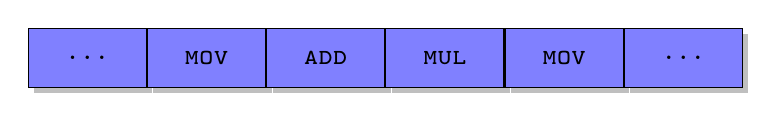
\begin{tikzpicture}[instruction/.style={font=\ttfamily\scshape,minimum height=.75cm,minimum width=1.5cm,draw,fill=blue!50,drop shadow}]
      \node[instruction] (instruction 1) {\dots};
      \node[instruction,anchor=north west] (instruction 2) at (instruction 1.north east) {mov};
      \node[instruction,anchor=north west] (instruction 3) at (instruction 2.north east) {add};
      \node[instruction,anchor=north west] (instruction 4) at (instruction 3.north east) {mul};
      \node[instruction,anchor=north west] (instruction 5) at (instruction 4.north east) {mov};
      \node[instruction,anchor=north west] (instruction 6) at (instruction 5.north east) {\dots};
    \end{tikzpicture}
  \end{center}
\end{frame}

\begin{frame}
  \frametitle{Car Assembly Analogy}
  \begin{itemize}
    \item Imagine car assembly line
    \item Assembling a car takes many phases
          \begin{itemize}
            \item E.g.~3 phases named A, B, C
          \end{itemize}
    \item Does it make sense to wait for one car to be finished before starting another?
    \item Assembly of 3 cars takes 9 time units
    \item Assembly of $n$ cars takes $3n$ steps
  \end{itemize}
  \begin{center}
    \begin{tikzpicture}[phase/.style={font=\scshape,minimum height=.75cm,minimum width=1cm},
                        phase a/.style={phase,fill=red!50},
                        phase b/.style={phase,fill=blue!50},
                        phase c/.style={phase,fill=green!50},]
      \node[phase a] (a1) {A};
      \node[phase b,anchor=north west] (b1) at (a1.north east) {B};
      \node[phase c,anchor=north west] (c1) at (b1.north east) {C};
      \node[phase a,anchor=north west] (a2) at (c1.north east) {A};
      \node[phase b,anchor=north west] (b2) at (a2.north east) {B};
      \node[phase c,anchor=north west] (c2) at (b2.north east) {C};
      \node[phase a,anchor=north west] (a3) at (c2.north east) {A};
      \node[phase b,anchor=north west] (b3) at (a3.north east) {B};
      \node[phase c,anchor=north west] (c3) at (b3.north east) {C};

      \foreach \i in {1,2,3} {
        \draw[|-|] ($ (a\i.south west) + (0,-0.1) $) -- ($ (c\i.south east) + (0,-0.1) $) node[midway,below,font=\small] {car \i};
      }

      \foreach[count=\i] \p in {a1,b1,c1,a2,b2,c2,a3,b3,c3} {
        \node[anchor=south,circle,draw,inner sep=1pt] at ($ (\p.north) + (0,0.1) $) {\tiny\i};
      }
    \end{tikzpicture}
  \end{center}
\end{frame}

\begin{frame}
  \frametitle{Car Assembly Analogy}
  \begin{itemize}
    \item Different phases of different cars can happen in parallel
    \item Start with car 2 as soon as car 1 finishes phase A
    \item Assembly of 3 cars takes 5 steps
    \item Assembly of $n$ cars takes $n+2$ steps
  \end{itemize}
  \begin{center}
    \begin{tikzpicture}[phase/.style={font=\scshape,minimum height=.75cm,minimum width=1cm},
                        phase a/.style={phase,fill=red!50},
                        phase b/.style={phase,fill=blue!50},
                        phase c/.style={phase,fill=green!50},]
      \node[phase a] (a1) {A};
      \node[phase b,anchor=north west] (b1) at (a1.north east) {B};
      \node[phase c,anchor=north west] (c1) at (b1.north east) {C};
      \node[phase a,anchor=north west] (a2) at (a1.south east) {A};
      \node[phase b,anchor=north west] (b2) at (b1.south east) {B};
      \node[phase c,anchor=north west] (c2) at (c1.south east) {C};
      \node[phase a,anchor=north west] (a3) at (a2.south east) {A};
      \node[phase b,anchor=north west] (b3) at (b2.south east) {B};
      \node[phase c,anchor=north west] (c3) at (c2.south east) {C};

      \foreach[count=\i] \pid in {a1,b1,c1,c2,c3} {
        \path let \p1=(a1.north), \p2=(\pid.north) in
              node[anchor=south,circle,draw,inner sep=1pt] at ($ (\x2,\y1) + (0,0.1) $) {\tiny\i};
      }
    \end{tikzpicture}
  \end{center}
\end{frame}

\begin{frame}
  \frametitle{Pipelining}
  \begin{itemize}
    \item Same approach is used by CPUs
    \item Instructions are split up in different stages (say 4)
    \item Different stages of different instructions execute in parallel
  \end{itemize}
  \vskip5mm
  \begin{overprint}
    \onslide<1>
    \begin{center}
      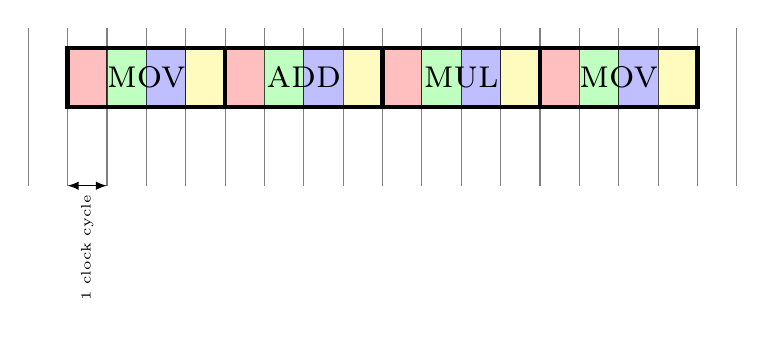
\begin{tikzpicture}[phase/.style={opacity=.5}]
        \foreach[evaluate={\i*0.5} as \x] \i in {-1,...,17} {
          \draw[gray,thin] (\x,-1) -- (\x,1);
        }

        \draw[latex-latex] (0,-1) -- (0.5,-1) node[rotate=90,left,midway,font=\tiny] {1 clock cycle};

        \foreach[count=\i,evaluate={(\i-1)*2} as \x] \instruction in {mov,add,mul,mov} {
          \begin{scope}[xshift=\x cm]
            \draw[phase,fill=red!50] (0,0) rectangle ++(0.5,0.75);
            \draw[phase,fill=green!50] (0.5,0) rectangle ++(0.5,0.75);
            \draw[phase,fill=blue!50] (1,0) rectangle ++(0.5,0.75);
            \draw[phase,fill=yellow!50] (1.5,0) rectangle ++(0.5,0.75);
            \draw[ultra thick] (0,0) rectangle ++(2,0.75);
            \node[font=\scshape] at (1,0.75/2) {\Large\instruction};
          \end{scope}
        }
      \end{tikzpicture}
    \end{center}

    \onslide<2>
    \begin{center}
      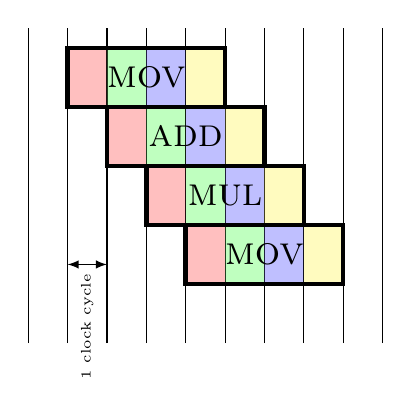
\begin{tikzpicture}[phase/.style={opacity=.5}]
        \foreach[evaluate={\i*0.5} as \x] \i in {-1,...,8} {
          \draw (\x,-3) -- (\x,1);
        }

        \draw[latex-latex] (0,-2) -- (0.5,-2) node[rotate=90,left,midway,font=\tiny] {1 clock cycle};

        \foreach[count=\i,evaluate={(\i-1)*0.5} as \x,evaluate={-(\i-1)*0.75} as \y] \instruction in {mov,add,mul,mov} {
          \begin{scope}[xshift=\x cm,yshift =\y cm]
            \draw[phase,fill=red!50] (0,0) rectangle ++(0.5,0.75);
            \draw[phase,fill=green!50] (0.5,0) rectangle ++(0.5,0.75);
            \draw[phase,fill=blue!50] (1,0) rectangle ++(0.5,0.75);
            \draw[phase,fill=yellow!50] (1.5,0) rectangle ++(0.5,0.75);
            \draw[ultra thick] (0,0) rectangle ++(2,0.75);
            \node[font=\scshape] at (1,0.75/2) {\Large\instruction};
          \end{scope}
        }
      \end{tikzpicture}
    \end{center}
  \end{overprint}
\end{frame}

\begin{frame}
  \frametitle{Pipelining}
  \begin{itemize}
    \item Allows instructions to overlap in time
    \item Instructions are executed in parallel
    \item To maximise efficiency, the pipeline needs to be fed new instructions at all times
  \end{itemize}
\end{frame}

\begin{frame}
  \frametitle{Conditionals}
  \code[language=c++14,width=.4\linewidth,font=\small]{conditional.cpp}
  \begin{itemize}
    \item Conditionals cause trouble
    \item \texttt{cond} determines which path to take
          \begin{itemize}
            \item We cannot add new instructions to pipeline as long as we don't know the value of \texttt{cond}
            \item Pipeline will be completely emptied before \texttt{a} or \texttt{b} executes
          \end{itemize}
    \item Really bad for performance
  \end{itemize}
\end{frame}

\begin{frame}
  \frametitle{Branch Prediction}
  \begin{itemize}
    \item Solution: try to guess which path will be taken
    \item CPU picks path and starts executing as if there was no \texttt{if}
    \item If chosen path turns out to be wrong path, CPU needs to undo everything
          \begin{itemize}
            \item Good performance if guess was good
            \item Bad performance if guess was bad
          \end{itemize}
    \item How does CPU maximise good guesses?
    \item Many different approaches possible
  \end{itemize}
\end{frame}

\begin{frame}
  \frametitle{Static Branch Prediction}
  \begin{itemize}
    \item CPU always guesses the then-branch will be taken
    \item Programmer needs to write program so that then-branch is more probable
  \end{itemize}
  \vskip5mm
  \begin{overprint}
    \onslide<1>
    \code[language=c++14,font=\small]{static-branch-prediction.cpp}

    \onslide<2>
    \code[language=c++14,font=\small]{static-branch-prediction2.cpp}
  \end{overprint}
\end{frame}

\begin{frame}
  \frametitle{Dynamic Branch Prediction}
  \begin{itemize}
    \item CPU keeps count at runtime
    \item Tries to detect patterns
  \end{itemize}
  \vskip5mm
  \begin{overprint}
    \onslide<1>
    \code[language=c++14,font=\small,width=.9\linewidth]{dynamic-branch-prediction.cpp}

    \onslide<2>
    \code[language=c++14,font=\small,width=.9\linewidth]{dynamic-branch-prediction2.cpp}
  \end{overprint}
\end{frame}

\begin{frame}
  \frametitle{Example Benchmark}
  \begin{center}
    \begin{tabular}{cc}
      \textbf{Pattern} & \textbf{Time} \\
      \toprule
      \texttt{F} & 5746 \\ % 0
      \texttt{FT} & 6264 \\ % 1
      \texttt{FFTT} & 5893 \\ % 2
      \texttt{FTTT} & 5808 \\ % 3
      \texttt{FFFTTTT} & 8692 \\ % 4
      \texttt{FTFTTTTT} & 7465 \\ % 5
      \texttt{FFTTTTTT} & 7832 \\ % 6
      \texttt{FTTTTTTTF} & 7059 \\ % 7
      \texttt{FFFFFFFFTTTTTTTT} & 8355 \\ % 8
      \texttt{FTFTFTFTTTTTTTTT} & 7814 \\ % 9
      \texttt{FFTTFFTTTTTTTTTT} & 7355 \\ % 10
      \texttt{FTTTFTTTTTTTTTTT} & 6931 \\ % 11
      \texttt{FFFFTTTTTTTTTTTT} & 7735 \\ % 12
    \end{tabular}
  \end{center}
  \begin{center} \bfseries
    Measurements done on Core i7 6700, 3.4GHz
  \end{center}
\end{frame}

%%% Local Variables:
%%% mode: latex
%%% TeX-master: "performance"
%%% End:

\section{Memory Alignment}

\frame{\tableofcontents[currentsection]}

\begin{frame}
  \frametitle{Reading from RAM}
  \begin{itemize}
    \item RAM is not organised as a series of bytes
    \item RAM is organised as a series of chunks
          \begin{itemize}
            \item For example, chunk of $4$ bytes long
          \end{itemize}
    \item Reading from RAM = reading one complete chunk
  \end{itemize}
  \begin{center}
    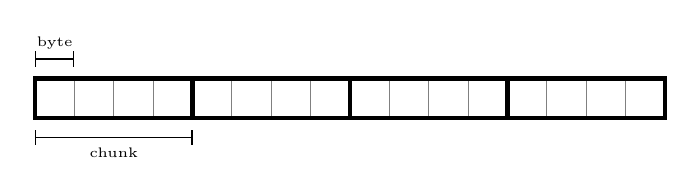
\begin{tikzpicture}
      \draw[thin,gray] (0,0) grid[xstep=0.5cm,ystep=0.5cm] (8,0.5);
      \draw[ultra thick] (0,0) grid[xstep=2cm,ystep=0.5cm] (8,0.5);
      \draw[ultra thick] (0,0) rectangle (8,0.5);

      \draw[|-|] (0,0.75) -- ++(0.5,0) node[midway,above,font=\tiny] {byte};
      \draw[|-|] (0,-0.25) -- ++(2,0) node[midway,below,font=\tiny] {chunk};
    \end{tikzpicture}
  \end{center}
\end{frame}

\begin{frame}
  \frametitle{Reading Aligned Block from RAM}
  \begin{center} \ttfamily\Large
    MOV EAX, [ESI]
  \end{center}
  \begin{center}
    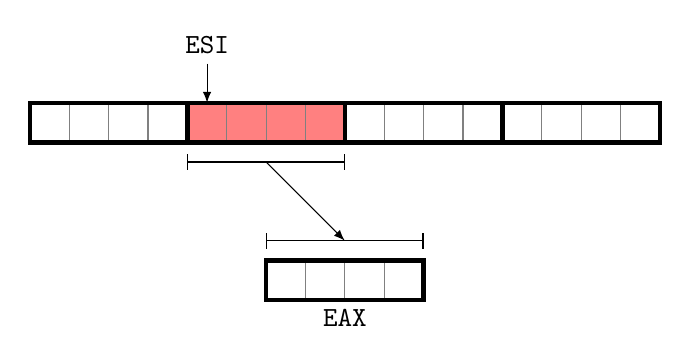
\begin{tikzpicture}
      \draw[fill=red!50] (2,0) rectangle ++(2,0.5);

      \draw[thin,gray] (0,0) grid[xstep=0.5cm,ystep=0.5cm] (8,0.5);
      \draw[ultra thick] (0,0) grid[xstep=2cm,ystep=0.5cm] (8,0.5);
      \draw[ultra thick] (0,0) rectangle (8,0.5);

      \draw[-latex] (2.25,1) -- ++(0,-0.5) node[above,at start,font=\ttfamily] {ESI};

      \draw[thin,gray] (3,-2) grid[xstep=0.5cm,ystep=0.5cm] ++(2,0.5);
      \draw[ultra thick] (3,-2) rectangle ++(2,0.5);

      \node[anchor=north,font=\ttfamily] at (4,-2) {EAX};

      \draw[|-|] (2,-0.25) -- ++(2,0);
      \draw[|-|] (3,-1.25) -- ++(2,0);
      \draw[-latex] (3,-0.25) -- (4,-1.25);
    \end{tikzpicture}
  \end{center}
  \begin{center}
    Reading a chunk from RAM to register happens in one step
  \end{center}
\end{frame}

\begin{frame}
  \frametitle{Reading Unaligned Block from RAM}
  \begin{center}
    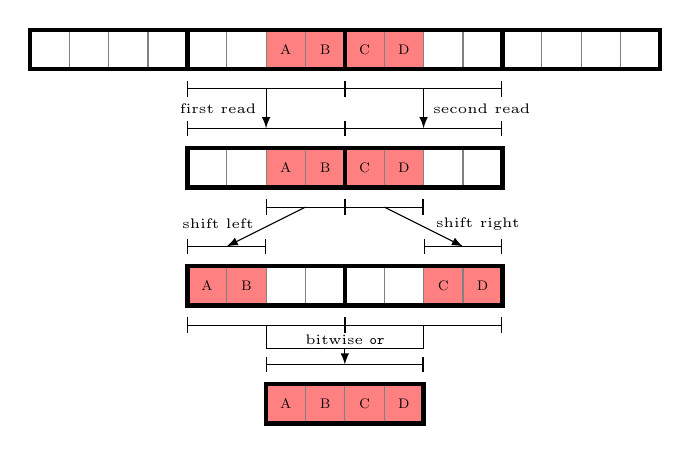
\begin{tikzpicture}[label/.style={font=\scshape\tiny}]
      \draw[fill=red!50] (3,0) rectangle ++(2,0.5);
      \draw[fill=red!50] (3,-1.5) rectangle ++(2,0.5);
      \draw[fill=red!50] (2,-3) rectangle ++(1,0.5);
      \draw[fill=red!50] (5,-3) rectangle ++(1,0.5);
      \draw[fill=red!50] (3,-4.5) rectangle ++(2,0.5);

      \draw[thin,gray] (0,0) grid[xstep=0.5cm,ystep=0.5cm] (8,0.5);
      \draw[ultra thick] (0,0) grid[xstep=2cm,ystep=0.5cm] (8,0.5);
      \draw[ultra thick] (0,0) rectangle (8,0.5);

      \draw[thin,gray] (2,-1.5) grid[xstep=0.5cm,ystep=0.5cm] ++(4,0.5);
      \draw[ultra thick] (2,-1.5) grid[xstep=2cm,ystep=0.5cm] ++(4,0.5);
      \draw[ultra thick] (2,-1.5) rectangle ++(4,0.5);

      \draw[thin,gray] (2,-3) grid[xstep=0.5cm,ystep=0.5cm] ++(4,0.5);
      \draw[ultra thick] (2,-3) grid[xstep=2cm,ystep=0.5cm] ++(4,0.5);
      \draw[ultra thick] (2,-3) rectangle ++(4,0.5);

      \draw[thin,gray] (3,-4.5) grid[xstep=0.5cm,ystep=0.5cm] ++(2,0.5);
      \draw[ultra thick] (3,-4.5) rectangle ++(2,0.5);

      \draw[|-|] (2,-0.25) -- ++(2,0);
      \draw[|-|] (2,-0.75) -- ++(2,0);
      \draw[-latex] (3,-0.25) -- (3,-0.75) node[left,font=\tiny,midway] {first read};

      \draw[|-|] (4,-0.25) -- ++(2,0);
      \draw[|-|] (4,-0.75) -- ++(2,0);
      \draw[-latex] (5,-0.25) -- (5,-0.75) node[right,font=\tiny,midway] {second read};

      \draw[|-|] (3,-1.75) -- ++(1,0);
      \draw[|-|] (2,-2.25) -- ++(1,0);
      \draw[-latex] (3.5,-1.75) -- (2.5,-2.25) node[left,font=\tiny,midway,xshift=-1pt,yshift=1pt] {shift left};

      \draw[|-|] (4,-1.75) -- ++(1,0);
      \draw[|-|] (5,-2.25) -- ++(1,0);
      \draw[-latex] (4.5,-1.75) -- (5.5,-2.25) node[right,font=\tiny,midway,xshift=1pt,yshift=1pt] {shift right};

      \draw[|-|] (2,-3.25) -- ++(2,0);
      \draw[|-|] (4,-3.25) -- ++(2,0);
      \draw[|-|] (3,-3.75) -- ++(2,0);
      \draw[-latex] (3,-3.25) -- ++(0,-0.3) -- ++(1,0) -- ++(0,-0.2);
      \draw (5,-3.25) -- ++(0,-0.3) -- ++(-1,0);
      \node[font=\tiny,anchor=south] at (4,-3.625) {bitwise \texttt{or}};

      \node[label] at (3.25,0.25) {A};
      \node[label] at (3.75,0.25) {B};
      \node[label] at (4.25,0.25) {C};
      \node[label] at (4.75,0.25) {D};

      \node[label] at (3.25,-1.25) {A};
      \node[label] at (3.75,-1.25) {B};
      \node[label] at (4.25,-1.25) {C};
      \node[label] at (4.75,-1.25) {D};

      \node[label] at (2.25,-2.75) {A};
      \node[label] at (2.75,-2.75) {B};
      \node[label] at (5.25,-2.75) {C};
      \node[label] at (5.75,-2.75) {D};

      \node[label] at (3.25,-4.25) {A};
      \node[label] at (3.75,-4.25) {B};
      \node[label] at (4.25,-4.25) {C};
      \node[label] at (4.75,-4.25) {D};
    \end{tikzpicture}
  \end{center}
  \begin{center}
    Reading 4 bytes that do not correspond to a chunk (i.e.~nonaligned) takes many steps
  \end{center}
\end{frame}

\begin{frame}
  \frametitle{Unaligned Memory Reads}
  \begin{itemize}
    \item If the word you need to read does not fit in one chunk, multiple reads will be necessary
    \item General rule of thumb: align $2^N$ sized words on a $2^N$-divisible memory address
          \begin{itemize}
            \item \texttt{uint8\_t} (1 byte long) can start anywhere
            \item \texttt{uint16\_t} (2 bytes) should start on address divisible by 2
            \item \texttt{uint32\_t} should start on address divisible by 4
            \item \texttt{uint64\_t} should start on address divisible by 8
          \end{itemize}
    \item This is generally done automatically by the compiler
  \end{itemize}
\end{frame}

\begin{frame}
  \frametitle{Size of Data Structures}
  \code[language=c++14]{sizeof.cpp}
  \begin{itemize}
    \item Should be $1+4+1+4 = 10$ bytes large
    \item \texttt{sizeof(Foo)} returns \texttt{16}
    \item Compiler leaves ``gaps'' so as to align \texttt{b} and \texttt{d} correctly
  \end{itemize}
\end{frame}

\begin{frame}
  \frametitle{\texttt{Foo} Memory Layout}
  \structure{Without Memory Alignment}
  \begin{center}
    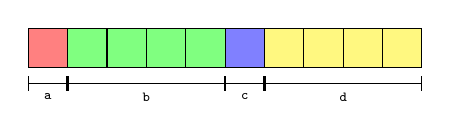
\begin{tikzpicture}
      \draw[fill=red!50] (0,0) rectangle ++(0.5,0.5);
      \draw[fill=green!50] (0.5,0) rectangle ++(2,0.5);
      \draw[fill=blue!50] (2.5,0) rectangle ++(0.5,0.5);
      \draw[fill=yellow!50] (3,0) rectangle ++(2,0.5);
      \draw[thin] (0,0) grid[xstep=0.5cm,ystep=0.5cm] ++(5,0.5);

      \begin{scope}[yshift=-2mm]
        \draw[|-|] (0,0) -- ++(0.5,0) node[midway,below,font=\tiny\ttfamily] {a};
        \draw[|-|] (0.5,0) -- ++(2,0) node[midway,below,font=\tiny\ttfamily] {b};
        \draw[|-|] (2.5,0) -- ++(0.5,0) node[midway,below,font=\tiny\ttfamily] {c};
        \draw[|-|] (3,0) -- ++(2,0) node[midway,below,font=\tiny\ttfamily] {d};
      \end{scope}
    \end{tikzpicture}
  \end{center}
  \structure{With Memory Alignment}
  \begin{center}
    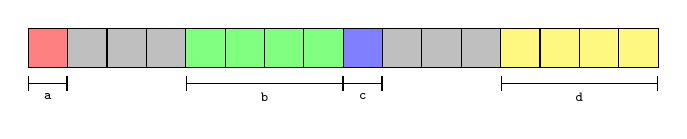
\begin{tikzpicture}
      \draw[fill=gray!50] (0,0) rectangle ++(8,0.5);
      \draw[fill=red!50] (0,0) rectangle ++(0.5,0.5);
      \draw[fill=green!50] (2,0) rectangle ++(2,0.5);
      \draw[fill=blue!50] (4,0) rectangle ++(0.5,0.5);
      \draw[fill=yellow!50] (6,0) rectangle ++(2,0.5);
      \draw[thin] (0,0) grid[xstep=0.5cm,ystep=0.5cm] ++(8,0.5);

      \begin{scope}[yshift=-2mm]
        \draw[|-|] (0,0) -- ++(0.5,0) node[midway,below,font=\tiny\ttfamily] {a};
        \draw[|-|] (2,0) -- ++(2,0) node[midway,below,font=\tiny\ttfamily] {b};
        \draw[|-|] (4,0) -- ++(0.5,0) node[midway,below,font=\tiny\ttfamily] {c};
        \draw[|-|] (6,0) -- ++(2,0) node[midway,below,font=\tiny\ttfamily] {d};
      \end{scope}
    \end{tikzpicture}
  \end{center}
  \begin{itemize}
    \item Grey: unused memory
    \item It would be better to rearrange members
          \begin{itemize}
            \item \texttt{a, c, b, d} would be optimal
            \item Compiler will always preserve order
            \item You need to rearrange yourself
          \end{itemize}
  \end{itemize}
\end{frame}

\begin{frame}
  \frametitle{Arrays}
  \begin{itemize}
    \item Extra complication: arrays
    \item We focused on aligning the members of one object
    \item What if we consider an array of such objects?
  \end{itemize}
\end{frame}

\begin{frame}
  \frametitle{Arrays}
  \code[language=c++14,font=\small,width=.5\linewidth]{int-char.cpp}
  \begin{center}
    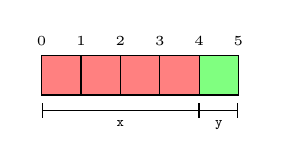
\begin{tikzpicture}
      \draw[fill=red!50] (0,0) rectangle ++(2,0.5);
      \draw[fill=green!50] (2,0) rectangle ++(0.5,0.5);
      \draw[thin] (0,0) grid[xstep=0.5cm,ystep=0.5cm] ++(2.5,0.5);

      \foreach[evaluate={\i*0.5} as \x] \i in {0,...,5} {
        \node[font=\tiny,anchor=south] at (\x,0.5) {\i};
      }

      \begin{scope}[yshift=-2mm]
        \draw[|-|] (0,0) -- ++(2,0) node[midway,below,font=\tiny\ttfamily] {x};
        \draw[|-|] (2,0) -- ++(0.5,0) node[midway,below,font=\tiny\ttfamily] {y};
      \end{scope}
    \end{tikzpicture}
  \end{center}
  \begin{itemize}
    \item Seems ok
    \item \texttt{x} is 4 bytes long and starts at 0
    \item \texttt{y} is 1 byte long, can start anywhere
    \item Members are aligned
  \end{itemize}
\end{frame}

\begin{frame}
  \frametitle{Arrays}
  \code[language=c++14,font=\small,width=.5\linewidth]{int-char.cpp}
  \begin{center}
    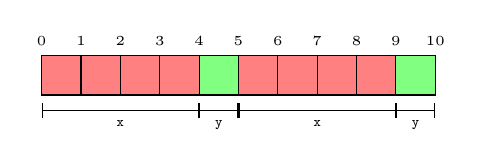
\begin{tikzpicture}
      \draw[fill=red!50] (0,0) rectangle ++(2,0.5);
      \draw[fill=green!50] (2,0) rectangle ++(0.5,0.5);
      \draw[fill=red!50] (2.5,0) rectangle ++(2,0.5);
      \draw[fill=green!50] (4.5,0) rectangle ++(0.5,0.5);
      \draw[thin] (0,0) grid[xstep=0.5cm,ystep=0.5cm] ++(5,0.5);

      \foreach[evaluate={\i*0.5} as \x] \i in {0,...,10} {
        \node[font=\tiny,anchor=south] at (\x,0.5) {\i};
      }

      \begin{scope}[yshift=-2mm]
        \draw[|-|] (0,0) -- ++(2,0) node[midway,below,font=\tiny\ttfamily] {x};
        \draw[|-|] (2,0) -- ++(0.5,0) node[midway,below,font=\tiny\ttfamily] {y};
        \draw[|-|] (2.5,0) -- ++(2,0) node[midway,below,font=\tiny\ttfamily] {x};
        \draw[|-|] (4.5,0) -- ++(0.5,0) node[midway,below,font=\tiny\ttfamily] {y};
      \end{scope}
    \end{tikzpicture}
  \end{center}
  \begin{itemize}
    \item Array of 2 \texttt{foo}s
    \item Second \texttt{foo}'s \texttt{x} starts at address \texttt{5}
    \item I.e.~it is not aligned correctly
  \end{itemize}
\end{frame}

\begin{frame}
  \frametitle{Arrays}
  \begin{itemize}
    \item To ensure that all members are aligned, even in arrays, add extra padding at end
    \item General rule:
          \begin{center}
            \alert{Total size must be a multiple of the largest member}
          \end{center}
    \item Largest member is \texttt{uint16\_t} $\rightarrow$ total size \% 2 = 0
    \item Largest member is \texttt{uint32\_t} $\rightarrow$ total size \% 4 = 0
  \end{itemize}
\end{frame}

\begin{frame}
  \frametitle{Example 1}
  \code[language=c++14,font=\ttfamily\small]{memalign-example1.cpp}
  \begin{overprint}
    \onslide<1|handout:1>
    \begin{center}
      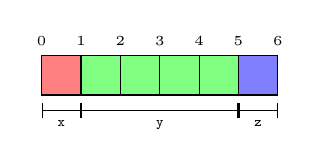
\begin{tikzpicture}
        \draw[fill=red!50] (0,0) rectangle ++(0.5,0.5);
        \draw[fill=green!50] (0.5,0) rectangle ++(2,0.5);
        \draw[fill=blue!50] (2.5,0) rectangle ++(0.5,0.5);
        \draw[thin] (0,0) grid[xstep=0.5cm,ystep=0.5cm] ++(3,0.5);

        \foreach[evaluate={\i*0.5} as \x] \i in {0,...,6} {
          \node[font=\tiny,anchor=south] at (\x,0.5) {\i};
        }

        \begin{scope}[yshift=-2mm]
          \draw[|-|] (0,0) -- ++(0.5,0) node[midway,below,font=\tiny\ttfamily] {x};
          \draw[|-|] (0.5,0) -- ++(2,0) node[midway,below,font=\tiny\ttfamily] {y};
          \draw[|-|] (2.5,0) -- ++(0.5,0) node[midway,below,font=\tiny\ttfamily] {z};
        \end{scope}
      \end{tikzpicture}
    \end{center}

    \onslide<2|handout:2>
    \begin{center}
      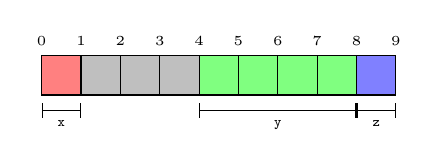
\begin{tikzpicture}
        \draw[fill=gray!50] (0,0) rectangle ++(4.5,0.5);
        \draw[fill=red!50] (0,0) rectangle ++(0.5,0.5);
        \draw[fill=green!50] (2,0) rectangle ++(2,0.5);
        \draw[fill=blue!50] (4,0) rectangle ++(0.5,0.5);
        \draw[thin] (0,0) grid[xstep=0.5cm,ystep=0.5cm] ++(4.5,0.5);

        \foreach[evaluate={\i*0.5} as \x] \i in {0,...,9} {
          \node[font=\tiny,anchor=south] at (\x,0.5) {\i};
        }

        \begin{scope}[yshift=-2mm]
          \draw[|-|] (0,0) -- ++(0.5,0) node[midway,below,font=\tiny\ttfamily] {x};
          \draw[|-|] (2,0) -- ++(2,0) node[midway,below,font=\tiny\ttfamily] {y};
          \draw[|-|] (4,0) -- ++(0.5,0) node[midway,below,font=\tiny\ttfamily] {z};
        \end{scope}
      \end{tikzpicture}
    \end{center}

    \onslide<3|handout:3>
    \begin{center}
      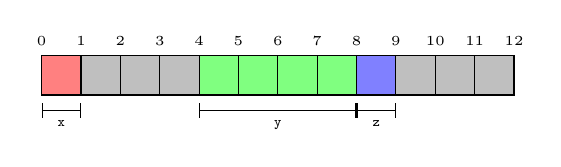
\begin{tikzpicture}
        \draw[fill=gray!50] (0,0) rectangle ++(6,0.5);
        \draw[fill=red!50] (0,0) rectangle ++(0.5,0.5);
        \draw[fill=green!50] (2,0) rectangle ++(2,0.5);
        \draw[fill=blue!50] (4,0) rectangle ++(0.5,0.5);
        \draw[thin] (0,0) grid[xstep=0.5cm,ystep=0.5cm] ++(6,0.5);

        \foreach[evaluate={\i*0.5} as \x] \i in {0,...,12} {
          \node[font=\tiny,anchor=south] at (\x,0.5) {\i};
        }

        \begin{scope}[yshift=-2mm]
          \draw[|-|] (0,0) -- ++(0.5,0) node[midway,below,font=\tiny\ttfamily] {x};
          \draw[|-|] (2,0) -- ++(2,0) node[midway,below,font=\tiny\ttfamily] {y};
          \draw[|-|] (4,0) -- ++(0.5,0) node[midway,below,font=\tiny\ttfamily] {z};
        \end{scope}
      \end{tikzpicture}
    \end{center}
  \end{overprint}
  \begin{overprint}
    \onslide<1|handout:1>
    \begin{center}
      Unaligned
    \end{center}

    \onslide<2|handout:2>
    \begin{center}
      Padding added to align members of single object
    \end{center}

    \onslide<3|handout:3>
    \begin{center}
      Adding padding to make total size a multiple of 4 \\
      This is final memory layout: \texttt{sizeof(Foo) == 12}
    \end{center}
  \end{overprint}
\end{frame}

\begin{frame}
  \frametitle{Example 2}
  \code[language=c++14,font=\ttfamily\small]{memalign-example2.cpp}
  \begin{overprint}
    \onslide<1|handout:1>
    \begin{center}
      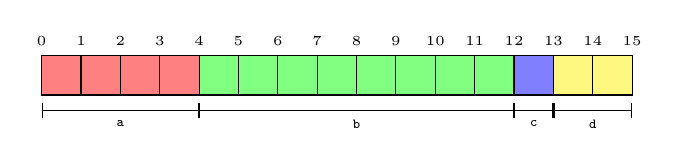
\begin{tikzpicture}
        \draw[fill=red!50] (0,0) rectangle ++(2,0.5);
        \draw[fill=green!50] (2,0) rectangle ++(4,0.5);
        \draw[fill=blue!50] (6,0) rectangle ++(0.5,0.5);
        \draw[fill=yellow!50] (6.5,0) rectangle ++(1,0.5);
        \draw[thin] (0,0) grid[xstep=0.5cm,ystep=0.5cm] ++(7.5,0.5);

        \foreach[evaluate={\i*0.5} as \x] \i in {0,...,15} {
          \node[font=\tiny,anchor=south] at (\x,0.5) {\i};
        }

        \begin{scope}[yshift=-2mm]
          \draw[|-|] (0,0) -- ++(2,0) node[midway,below,font=\tiny\ttfamily] {a};
          \draw[|-|] (2,0) -- ++(4,0) node[midway,below,font=\tiny\ttfamily] {b};
          \draw[|-|] (6,0) -- ++(0.5,0) node[midway,below,font=\tiny\ttfamily] {c};
          \draw[|-|] (6.5,0) -- ++(1,0) node[midway,below,font=\tiny\ttfamily] {d};
        \end{scope}
      \end{tikzpicture}
    \end{center}

    \onslide<2|handout:2>
    \begin{center}
      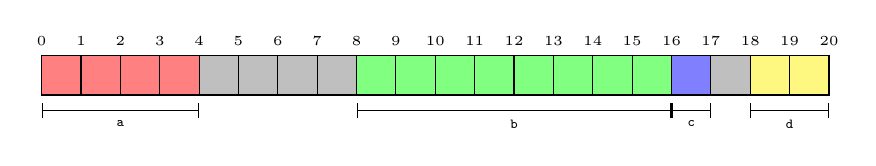
\begin{tikzpicture}
        \draw[fill=gray!50] (0,0) rectangle ++(10,0.5);
        \draw[fill=red!50] (0,0) rectangle ++(2,0.5);
        \draw[fill=green!50] (4,0) rectangle ++(4,0.5);
        \draw[fill=blue!50] (8,0) rectangle ++(0.5,0.5);
        \draw[fill=yellow!50] (9,0) rectangle ++(1,0.5);
        \draw[thin] (0,0) grid[xstep=0.5cm,ystep=0.5cm] ++(10,0.5);

        \foreach[evaluate={\i*0.5} as \x] \i in {0,...,20} {
          \node[font=\tiny,anchor=south] at (\x,0.5) {\i};
        }

        \begin{scope}[yshift=-2mm]
          \draw[|-|] (0,0) -- ++(2,0) node[midway,below,font=\tiny\ttfamily] {a};
          \draw[|-|] (4,0) -- ++(4,0) node[midway,below,font=\tiny\ttfamily] {b};
          \draw[|-|] (8,0) -- ++(0.5,0) node[midway,below,font=\tiny\ttfamily] {c};
          \draw[|-|] (9,0) -- ++(1,0) node[midway,below,font=\tiny\ttfamily] {d};
        \end{scope}
      \end{tikzpicture}
    \end{center}

    \onslide<3|handout:3>
    \begin{center}
      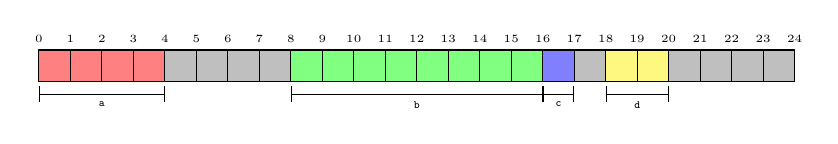
\begin{tikzpicture}[scale=.8,transform shape]
        \draw[fill=gray!50] (0,0) rectangle ++(12,0.5);
        \draw[fill=red!50] (0,0) rectangle ++(2,0.5);
        \draw[fill=green!50] (4,0) rectangle ++(4,0.5);
        \draw[fill=blue!50] (8,0) rectangle ++(0.5,0.5);
        \draw[fill=yellow!50] (9,0) rectangle ++(1,0.5);
        \draw[thin] (0,0) grid[xstep=0.5cm,ystep=0.5cm] ++(12,0.5);

        \foreach[evaluate={\i*0.5} as \x] \i in {0,...,24} {
          \node[font=\tiny,anchor=south] at (\x,0.5) {\i};
        }

        \begin{scope}[yshift=-2mm]
          \draw[|-|] (0,0) -- ++(2,0) node[midway,below,font=\tiny\ttfamily] {a};
          \draw[|-|] (4,0) -- ++(4,0) node[midway,below,font=\tiny\ttfamily] {b};
          \draw[|-|] (8,0) -- ++(0.5,0) node[midway,below,font=\tiny\ttfamily] {c};
          \draw[|-|] (9,0) -- ++(1,0) node[midway,below,font=\tiny\ttfamily] {d};
        \end{scope}
      \end{tikzpicture}
    \end{center}
  \end{overprint}
  \begin{overprint}
    \onslide<1|handout:1>
    \begin{center}
      Unaligned
    \end{center}

    \onslide<2|handout:2>
    \begin{center}
      Padding added to align members of single object
    \end{center}

    \onslide<3|handout:3>
    \begin{center}
      Adding padding to make total size a multiple of 8 \\
      This is final memory layout: \texttt{sizeof(Foo) == 24}
    \end{center}
  \end{overprint}
\end{frame}


\begin{frame}
  \frametitle{Benchmark: Reading \texttt{uint64\_t}}
  \begin{center}
    \begin{tabular}{cc}
      \textbf{Memory Address} & \textbf{Time} \\
      \toprule
      $8k+0$ & 2189 \\
      $8k+1$ & 3506 \\
      $8k+2$ & 3524 \\
      $8k+3$ & 3611 \\
      $8k+4$ & 3605 \\
      $8k+5$ & 3560 \\
      $8k+6$ & 3566 \\
      $8k+7$ & 3547 \\
    \end{tabular}
  \end{center}
\end{frame}

%%% Local Variables:
%%% mode: latex
%%% TeX-master: "performance"
%%% End:

\section{Cache}

\frame{\tableofcontents[currentsection]}


\begin{frame}
  \frametitle{\only<1-5>{Your Work Environment}\only<6>{Storage Mediums}}
  \begin{center}
    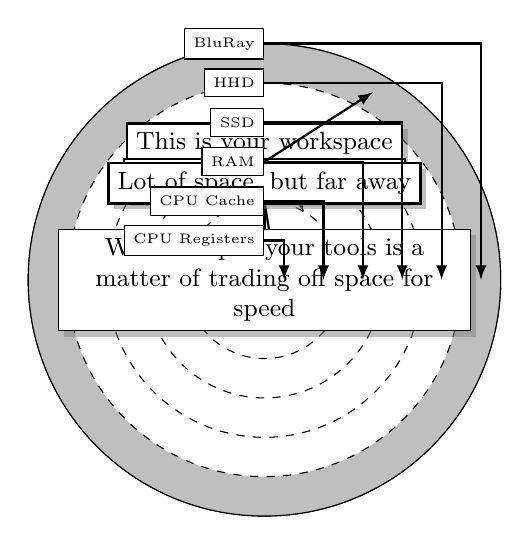
\begin{tikzpicture}[message/.style={fill=white,draw,font=\small,text opacity=1,drop shadow},
                        arrow/.style={black,thick,-latex}]
      \pgfdeclarelayer{background}
      \pgfdeclarelayer{foreground}
      \pgfsetlayers{background,main,foreground}

      \draw (0,0) circle [radius=3 cm];

      \draw[fill=black] (0,0) circle [radius=0.05cm];

      \begin{pgfonlayer}{foreground}
        \visible<1>{
          \draw[arrow] (90:1.25) -- (90:0.1) node[black,message,at start,above] {This is you};
        }

        \visible<2>{
          \draw[arrow] (90:2) -- (60:1) node[black,message,at start,below] {This is your workspace};
        }

        \visible<3>{
          \draw[arrow] (90:1) -- (60:0.25) node[black,message,at start,above] {Nearby, but little space};
        }

        \visible<4>{
          \draw[arrow] (90:1.5) -- (60:2.75) node[black,message,at start,below] {Lot of space, but far away};
        }

        \visible<5>{
          \node[message] at (0,0) {
            \parbox{5cm}{
              \centering Where to put your tools is a matter of trading off space for speed
            }};
        }

        \visible<6>{
          \foreach[count=\i,evaluate={\i*0.5-0.25} as \x,evaluate={\i*0.5} as \y] \medium in {CPU Registers,CPU Cache,RAM,SSD,HHD,BluRay} {
            \node[draw,fill=white,anchor=east,font=\tiny] (medium) at (0,\y) {\medium};
            \draw[-latex,thick] (medium) -| (\x,0);
          }
        }
      \end{pgfonlayer}

      \onslide<3->{
        \foreach[count=\i,evaluate={\r/3*100} as \x] \r in {2.5,2,...,0.5} {
          \draw[dashed] (0,0) circle [radius=\r cm];
        }
      }

      \begin{pgfonlayer}{background}
        \onslide<2>{
          \draw[fill=gray!50] (0,0) circle [radius=3cm];
        }

        \onslide<3>{
          \fill[gray!50] (0,0) circle [radius=0.5cm];
        }

        \onslide<4>{
          \fill[gray!50] (0,0) circle [radius=3cm];
          \fill[white] (0,0) circle [radius=2.5cm];
        }
      \end{pgfonlayer}
    \end{tikzpicture}
  \end{center}
\end{frame}

\begin{frame}
  \frametitle{Caching}
  \begin{itemize}
    \item Cheap storage is often slow
    \item Most often used data on fast storage medium
    \item Least often used data on cheap storage medium
  \end{itemize}
  \begin{center}
    \begin{tabular}{lc}
      \textbf{Storage} & \textbf{Speed (GB/s)} \\
      \toprule
      BluRay & 0.027 \\
      HDD & 0.15 \\
      SSD & \SI{3}{} \\
      RAM & \SI{30}{} \\
      L1 Cache & \SI{1000}{} \\
      CPU Registers & \SI{30000}{}
    \end{tabular}
  \end{center}
\end{frame}

\begin{frame}
  \frametitle{CPU Cache}
  \begin{itemize}
    \item CPU registers are blazingly fast
    \item RAM is relatively slow compared to CPU
    \item Cache bridges the speed gap
    \item How does it do that?
    \item Optimisation is always a matter of making assumptions
  \end{itemize}
\end{frame}

\subsection{Temporal Locality}

\frame{\tableofcontents[currentsubsection]}

\begin{frame}
  \frametitle{Temporal Locality}
  \begin{itemize}
    \item Assumption: code often accesses same memory locations repeatedly in short time
    \item Opposite of: code accesses some memory location once, and then leaves it alone for a long time
    \item This idea is known as \emph{temporal locality}
    \item How to make use of temporal locality?
  \end{itemize}
\end{frame}

\begin{frame}
  \frametitle{Cache (Simplified Explanation)}
  \begin{center}
    \begin{tikzpicture}[part/.style={draw,minimum width=1.5cm,minimum height=.5cm,font=\small\scshape},
                        cpu/.style={part,fill=blue!50},
                        cache/.style={part,fill=green!50},
                        ram/.style={part,fill=red!50},
                        fetch/.style={-latex,thick},
                        slow fetch/.style={fetch,red},
                        fast fetch/.style={fetch,green!50!black},
                        caption/.style={font=\small\scshape}]
      \pgfdeclarelayer{background}
      \pgfdeclarelayer{foreground}
      \pgfsetlayers{background,main,foreground}

      \node[cpu] (cpu) at (0,0) {cpu};

      \node[cache] (cache line 1) at (2.5,0.9) {\only<5-10>{a}\only<11-19>{e}\only<20->{d}};
      \node[cache] (cache line 2) at (2.5,0.3) {\only<8-13>{b}\only<14->{a}};
      \node[cache] (cache line 3) at (2.5,-0.3) {\only<8-15>{c}\only<16->{b}};
      \node[cache] (cache line 4) at (2.5,-0.9) {\only<8-17>{d}\only<18->{c}};

      \node[ram] (ram 1) at (8,1.5) {a};
      \node[ram] (ram 2) at (8,0.9) {b};
      \node[ram] (ram 3) at (8,0.3) {c};
      \node[ram] (ram 4) at (8,-0.3) {d};
      \node[ram] (ram 5) at (8,-0.9) {e};
      \node[ram] (ram 6) at (8,-1.5) {f};
      \node[anchor=south,inner sep=0mm,yshift=5pt] (ram above) at (ram 1.north) {\vdots};
      \node[anchor=north,inner sep=0mm] (ram below) at (ram 6.south) {\vdots};

      \begin{pgfonlayer}{background}
        \draw[fill=green!25] let \p1=(cache line 1.north west),
                                 \p2=(cache line 4.south east)
                             in
                             ($ (\x1,\y1) + (-0.25,0.25) $) coordinate (cache upper left)
                             rectangle
                             ($ (\x2,\y2) + (0.25,-0.25) $) coordinate (cache lower right);

        \path let \p1=(cache upper left),
                  \p2=($ (cache upper left) ! 0.5 ! (cache lower right) $),
                  \p3=(cache lower right)
              in
              coordinate (cache center) at (\p2)
              coordinate (cache left) at (\x1,\y2)
              coordinate (cache right) at (\x3,\y2);

        \draw[fill=red!25] let \p1=(ram 1.north west),
                               \p2=(ram 1.south east),
                               \p3=(ram above.north west),
                               \p4=(ram below.south east)
                           in
                           ($ (\x1,\y3) + (-0.25,0.25) $)
                           rectangle
                           ($ (\x2,\y4) + (0.25,-0.25) $);

        \path let \p1=($ (cache line 1.north west) ! 0.5 ! (cache line 4.south east) $),
                  \p2=(cache line 4)
              in
              node[anchor=north,caption] at (\x1,\y2-0.5cm) {cache};
        \path let \p1=($ (ram 1.north west) ! 0.5 ! (ram 6.south east) $),
                  \p2=(ram below.south east)
              in
              node[anchor=north,caption] at (\x1,\y2-0.25cm) {ram};
      \end{pgfonlayer}

      \visible<3>{
        \draw[fast fetch] (cpu) -- (cache left) node[above,midway,font=\tiny] {read A};
      }

      \visible<4>{
        \draw[slow fetch] (cache right) -- ++(0.5,0) |- (ram 1);
      }

      \visible<5>{
        \draw[slow fetch] (ram 1.west) -- ++(-0.75,0) |- (cache line 1.east);
        \draw[fast fetch] (cache line 1.west) -- ++(-0.5,0) |- (cpu);
      }

      \visible<6>{
        \draw[fast fetch] (cpu) -- (cache left) node[above,midway,font=\tiny] {read A};
      }

      \visible<7>{
        \draw[fast fetch] (cache line 1.west) -- ++(-0.5,0) |- (cpu);
      }

      \visible<10>{
        \draw[fast fetch] (cpu) -- (cache left) node[above,midway,font=\tiny] {read E};
      }

      \visible<11>{
        \draw[slow fetch] (ram 5.west) -- ++(-0.75,0) |- (cache line 1.east);
        \draw[fast fetch] (cache line 1.west) -- ++(-0.5,0) |- (cpu);
      }

      \visible<13>{
        \draw[fast fetch] (cpu) -- (cache left) node[above,midway,font=\tiny] {read A};
      }

      \visible<14>{
        \draw[slow fetch] (ram 1.west) -- ++(-0.75,0) |- (cache line 2.east);
        \draw[fast fetch] (cache line 2.west) -- ++(-0.5,0) |- (cpu);
      }

      \visible<15>{
        \draw[fast fetch] (cpu) -- (cache left) node[above,midway,font=\tiny] {read B};
      }

      \visible<16>{
        \draw[slow fetch] (ram 2.west) -- ++(-0.75,0) |- (cache line 3.east);
        \draw[fast fetch] (cache line 3.west) -- ++(-0.5,0) |- (cpu);
      }

      \visible<17>{
        \draw[fast fetch] (cpu) -- (cache left) node[above,midway,font=\tiny] {read C};
      }

      \visible<18>{
        \draw[slow fetch] (ram 3.west) -- ++(-0.75,0) |- (cache line 4.east);
        \draw[fast fetch] (cache line 4.west) -- ++(-0.5,0) |- (cpu);
      }

      \visible<19>{
        \draw[fast fetch] (cpu) -- (cache left) node[above,midway,font=\tiny] {read D};
      }

      \visible<20>{
        \draw[slow fetch] (ram 4.west) -- ++(-0.75,0) |- (cache line 1.east);
        \draw[fast fetch] (cache line 1.west) -- ++(-0.5,0) |- (cpu);
      }
    \end{tikzpicture}
  \end{center}
  \begin{overprint}
    \onslide<2|handout:2>
    \begin{center}
      Say cache can contain 4 lines
    \end{center}

    \onslide<3|handout:3>
    \begin{center}
      CPU wants to read RAM location A
    \end{center}

    \onslide<4|handout:4>
    \begin{center}
      Cache is empty at this point \\ We need to wait for RAM to answer
    \end{center}

    \onslide<5|handout:5>
    \begin{center}
      After a few cycles, RAM answers \\
      Result is copied to cache
    \end{center}

    \onslide<6|handout:6>
    \begin{center}
      CPU wants to read A again \\
    \end{center}

    \onslide<7|handout:7>
    \begin{center}
      A is already in cache; CPU receives answer quickly \\
      All subsequent reads to A will be fast
    \end{center}

    \onslide<8|handout:8>
    \begin{center}
      Say CPU reads B, C, D, then cache will look like this
    \end{center}

    \onslide<9|handout:9>
    \begin{center}
      If CPU keeps working on A, B, C, D, everything will go fast
    \end{center}

    \onslide<10|handout:10>
    \begin{center}
      What if the CPU now wants to read E?
    \end{center}

    \onslide<11|handout:11>
    \begin{center}
      Cache is full so one of its lines needs to be recycled \\
      Let's say the oldest one (A) is sacrificed
    \end{center}

    \onslide<12|handout:12>
    \begin{center}
      As long as CPU restricts itself to B, C, D, E, \\
      everything will be fine
    \end{center}

    \onslide<13-20|handout:13-20>
    \begin{center}
      What if the CPU now starts reading A, B, C, D, E cyclically?
    \end{center}

    \onslide<21|handout:21>
    \begin{center}
      This is disastrous as all reads will be slow
    \end{center}
  \end{overprint}
\end{frame}

\begin{frame}
  \frametitle{Cache}
  \begin{itemize}
    \item For cache to work well, it is important that CPU keeps accessing the same memory locations
    \item If CPU jumps around too much, cache lines will be recycled each time and performance
          will be as bad as if there is no cache
  \end{itemize}
\end{frame}

\begin{frame}
  \frametitle{Benchmark}
  \structure{Setup}
  \begin{itemize}
    \item We start with large block of memory
    \item We split this memory up in $N$ blocks
    \item For each block in turn, we access its contents $k$ times
  \end{itemize}
  \vskip5mm
  \structure{Expectations}
  \begin{itemize}
    \item First block access will be slowest (not yet in cache)
    \item Subsequent access should be fast, if block fits in cache
    \item If block too large, even subsequent access should be slow
  \end{itemize}
\end{frame}

\begin{frame}
  \frametitle{Benchmark}
  \begin{center}
    \begin{tikzpicture}
      \tikzmath{
        real \xdiv;
        real \ydiv;
        \xdiv=2;
        \ydiv=600;
      }
      \draw[thin,gray] (0,0) grid (10,6);
      \foreach[evaluate={\i/\xdiv} as \x,
               evaluate={\j/\ydiv} as \y,
               remember=\x as \lastx (initially 0),
               remember=\y as \lasty (initially 0)] \i/\j in
               {1/796,
                2/1001,
                3/1016,
                4/892,
                5/832,
                6/808,
                7/806,
                8/890,
                9/823,
                10/809,
                11/831,
                12/895,
                13/870,
                14/872,
                15/959,
                16/1033,
                17/1829,
                18/2906,
                19/3308} {
        \ifnum\i>1
          \draw[red] (\lastx,\lasty) -- (\x,\y);
        \fi
      }

      \foreach[evaluate={\i/\xdiv} as \x,
               evaluate={\j/\ydiv} as \y,
               remember=\x as \lastx (initially 0),
               remember=\y as \lasty (initially 0)] \i/\j in
               {1/744,
                2/848,
                3/865,
                4/791,
                5/755,
                6/749,
                7/751,
                8/769,
                9/767,
                10/792,
                11/788,
                12/775,
                13/790,
                14/824,
                15/816,
                16/997,
                17/1732,
                18/2665,
                19/3084} {
        \ifnum\i>1
          \draw[green] (\lastx,\lasty) -- (\x,\y);
        \fi
      }

      \foreach[evaluate={\i/\xdiv} as \x,
               evaluate={\j/\ydiv} as \y,
               remember=\x as \lastx (initially 0),
               remember=\y as \lasty (initially 0)] \i/\j in
               {1/729,
                2/793,
                3/783,
                4/771,
                5/770,
                6/731,
                7/758,
                8/736,
                9/750,
                10/780,
                11/737,
                12/748,
                13/767,
                14/786,
                15/789,
                16/807,
                17/1460,
                18/2620,
                19/3046} {
        \ifnum\i>1
          \draw[blue] (\lastx,\lasty) -- (\x,\y);
        \fi
      }

      \foreach[evaluate={\i/\xdiv} as \x,
      evaluate={\j/\ydiv} as \y,
               remember=\x as \lastx (initially 0),
               remember=\y as \lasty (initially 0)] \i/\j in
               {1/728,
                2/754,
                3/745,
                4/728,
                5/721,
                6/717,
                7/718,
                8/721,
                9/723,
                10/733,
                11/729,
                12/726,
                13/742,
                14/769,
                15/784,
                16/802,
                17/1449,
                18/2616,
                19/3120} {
        \ifnum\i>1
          \draw[purple] (\lastx,\lasty) -- (\x,\y);
        \fi
      }
    \end{tikzpicture}
  \end{center}
\end{frame}

\subsection{Spatial Locality}

\frame{\tableofcontents[currentsubsection]}

\begin{frame}
  \frametitle{Spatial Locality}
  \begin{itemize}
    \item Other typical usage pattern
    \item CPU often access memory range sequentially
          \begin{itemize}
            \item E.g.~accessing all elements in an array one after the other
          \end{itemize}
    \item How to make use of this?
  \end{itemize}
\end{frame}

\begin{frame}
  \frametitle{Prefetching}
  \begin{itemize}
    \item When CPU starts accessing memory locations \texttt{p}, \texttt{p+1}, \texttt{p+2},
          already ask RAM for \texttt{p+10}
    \item By the time CPU is done processing \texttt{p}\dots\texttt{p+9}, the rest of the
          data has already been fetched from RAM
  \end{itemize}
\end{frame}

\begin{frame}
  \frametitle{Benchmark}
  \begin{itemize}
    \item Accessing array sequentially: \SI{77}{\milli\second}
    \item Accessing array at random indices: \SI{1848}{\milli\second}
  \end{itemize}
\end{frame}


%%% Local Variables:
%%% mode: latex
%%% TeX-master: "performance"
%%% End:




%%% Local Variables:
%%% mode: latex
%%% TeX-master: "performance"
%%% End:

\section{Compiler Optimisations}

\frame{\tableofcontents[currentsection]}

\begin{frame}
  \frametitle{Compiler Optimisations}
  \begin{itemize}
    \item Compiler does not translate your code verbatim
    \item Compiler only promises to generate code that behaves the same as your code
    \item Compiler knows CPU better than you
    \item Compiler will transform your code so that it runs faster
    \item Compiler has many tricks up its sleeve
  \end{itemize}
\end{frame}


\subsection{Dead Code Elimination}

\frame{\tableofcontents[currentsubsection]}

\begin{frame}
  \frametitle{Dead Code Elimination}
  \begin{itemize}
    \item Dead code = code that will never be executed
    \item Compiler removes dead code
    \item Code below gets compiled to nothing
  \end{itemize}
  \code[language=c++14,font=\small,width=.6\linewidth]{dead-code.cpp}
\end{frame}



%%% Local Variables:
%%% mode: latex
%%% TeX-master: "performance"
%%% End:

\subsection{Inlining}

\frame{\tableofcontents[currentsubsection]}

\begin{frame}
  \frametitle{Inlining}
  \begin{itemize}
    \item Calling a function incurs some overhead
            \begin{itemize}
              \item Save important register values
              \item Prepare parameters
              \item \texttt{CALL}
              \item Execute body
              \item Prepare return value
              \item \texttt{RET}
              \item Restore important register values
            \end{itemize}
    \item This overhead should remain small compared to time needed for actual body
    \item This isn't the case with small functions
          \begin{itemize}
            \item E.g.~getters
          \end{itemize}
  \end{itemize}
\end{frame}

\begin{frame}
  \frametitle{Inlining}
  \begin{itemize}
    \item Inlining copies the body of the callee into the caller's body
  \end{itemize}
  \code[language=c++14,font=\small,width=.5\linewidth]{inlining.cpp}
\end{frame}

\begin{frame}
  \frametitle{Inlining}
  \begin{itemize}
    \item Inlining is good for short functions
    \item Could be bad for cache
          \begin{itemize}
            \item Cache works best if same code is executed often
            \item Inlining make copies, each called once
          \end{itemize}
    \item Compiler can be smart enough to dispense with pointers/references
  \end{itemize}
\end{frame}

\begin{frame}
  \frametitle{Inlining: Example}
  \code[language=c++14,font=\small]{swap.cpp}
  \begin{center}
    is compiled to
  \end{center}
  \code[font=\small,width=.25\linewidth]{swap.asm}
  \begin{itemize}
    \item Notice lack of \texttt{CALL}/\texttt{RET}
    \item Notice lack of pointer
  \end{itemize}
\end{frame}



%%% Local Variables:
%%% mode: latex
%%% TeX-master: "performance"
%%% End:

\subsection{Zero Cost Abstractions}

\frame{\tableofcontents[currentsubsection]}

\begin{frame}
  \frametitle{Zero Cost Abstractions}
  \begin{itemize}
    \item Similarly to inlining, objects can be compiled away
    \item If a \texttt{Foo} contains only a \texttt{double}, working with a \texttt{Foo} is as fast as working with a \texttt{double}
    \item There is no inherent overhead to objects
  \end{itemize}
\end{frame}

\begin{frame}
  \frametitle{Example: Angles}
  \begin{itemize}
    \item Angles can be represented by \texttt{double}s
    \item Is given \texttt{double} an angle expressed in radians or degrees?
    \item No way of knowing
  \end{itemize}
\end{frame}

\begin{frame}
  \frametitle{Example: Angles}
  \begin{itemize}
    \item We introduce helper class \texttt{angle}
  \end{itemize}
  \code[language=c++14,font=\small]{angle.cpp}
\end{frame}

\begin{frame}
  \frametitle{Example: Angles}
  \begin{itemize}
    \item Type contains the unit (\texttt{rad}/\texttt{deg})
    \item No mistakes possible, compiler will catch them
    \item Is just as fast as working with straight \texttt{double}s
  \end{itemize}
  \code[language=c++14,font=\small]{angle-usage.cpp}
\end{frame}


%%% Local Variables:
%%% mode: latex
%%% TeX-master: "performance"
%%% End:

\subsection{Compile Time Execution}

\frame{\tableofcontents[currentsubsection]}

\begin{frame}
  \frametitle{Compile Time Execution}
  \begin{itemize}
    \item Compiler can choose to execute code itself
    \item The resulting executable then does contain the computation, but only the result
  \end{itemize}
\end{frame}

\begin{frame}
  \frametitle{Example 1}
  \code[language=c++14,font=\small]{sum.cpp}
  \begin{center}
    gets compiled to
  \end{center}
  \code[width=.4\linewidth]{sum.asm}
\end{frame}

\begin{frame}
  \frametitle{Example 2}
  \code[language=c++14,font=\small,width=.9\linewidth]{count-rt.cpp}
  \vskip-5mm
  \begin{itemize}
    \item Using inheritance (\`a la Java)
    \item Time used: \SI{2020}{\milli\second}
  \end{itemize}
\end{frame}

\begin{frame}
  \frametitle{Example 2}
  \code[language=c++14,font=\small]{count-ct.cpp}
  \vskip-5mm
  \begin{itemize}
    \item Using templates forces things to be compile time
    \item Time used: \SI{571}{\milli\second}, i.e. 4$\times$ faster
  \end{itemize}
\end{frame}


%%% Local Variables:
%%% mode: latex
%%% TeX-master: "performance"
%%% End:

\subsection{Tail Call Optimisation}

\frame{\tableofcontents[currentsubsection]}

\begin{frame}
  \frametitle{Tail Call Optimisation}
  \begin{itemize}
    \item Recursive functions call themselves
          \begin{itemize}
            \item Involves \texttt{CALL}, \texttt{RET}
            \item Involves \texttt{PUSH} and \texttt{POP}
          \end{itemize}
    \item Are iterative approaches (= using loops) more efficient?
          \begin{itemize}
            \item Reuse of same local variables instead of always new ones
            \item No \texttt{CALL} or \texttt{RET} needed
          \end{itemize}
  \end{itemize}
\end{frame}

\begin{frame}
  \frametitle{Tail Call Optimisation}
  \code[language=c++14,font=\small,width=.7\linewidth]{tail-call.cpp}
  \begin{itemize}
    \item Tail call = returning result of recursive call without any postprocessing
          \begin{itemize}
            \item \texttt{return rec()} is ok
            \item \texttt{return 1 + rec()} is not ok
          \end{itemize}
    \item Multiple \texttt{return}s allowed, as long as they are all tail calls
    \item Recursive call can then recycle same locals
          \begin{itemize}
            \item No new stack frame needed for recursive call
            \item Just reuse current one
          \end{itemize}
    \item Tail Call Optimisation transforms recursion to loop
  \end{itemize}
\end{frame}

\begin{frame}
  \frametitle{Tail Call Optimisation: Example}
  \code[language=c++14,font=\small]{find-last.cpp}
  \begin{center}
    Recursive algorithm
  \end{center}
\end{frame}

\begin{frame}
  \frametitle{Tail Call Optimisation: Example}
  \code[font=\small,width=.99\linewidth]{find-last.asm}
  \begin{center}
    Generated assembly is iterative
  \end{center}
\end{frame}


%%% Local Variables:
%%% mode: latex
%%% TeX-master: "performance"
%%% End:

\section{Loop Optimisations}

\frame{\tableofcontents[currentsection]}

\begin{frame}
  \frametitle{Loop Optimisations}
  \begin{itemize}
    \item Loops can be rewritten in many ways
    \item Loops are perfect candidates for optimisation
          \begin{itemize}
            \item Most of execution time is spent in loops
          \end{itemize}
    \item Loops can be rewritten so as to
          \begin{itemize}
            \item Reduce loop overhead
            \item Improve locality
          \end{itemize}
  \end{itemize}
\end{frame}

\begin{frame}
  \frametitle{\link{https://en.wikipedia.org/wiki/Loop_unrolling}{Loop Unrolling}}
  \code[language=c++14,font=\small]{loop-unrolling.cpp}
  \vskip-5mm
  \begin{itemize}
    \item Reduces amount of loop condition checks
  \end{itemize}
\end{frame}

\begin{frame}
  \frametitle{\link{https://en.wikipedia.org/wiki/Loop_fission}{Loop Fission}}
  \code[language=c++14,font=\small]{loop-fission.cpp}
  \vskip-5mm
  \begin{itemize}
    \item Before: CPU hops back and forth in memory
    \item After: goes linearly over elements; better for cache
  \end{itemize}
\end{frame}

\begin{frame}
  \frametitle{\link{https://en.wikipedia.org/wiki/Loop_interchange}{Loop Interchange}}
  \code[language=c++14,font=\small]{loop-interchange.cpp}
  \vskip-5mm
  \begin{itemize}
    \item Before: CPU hops around a lot
    \item After: CPU processes each array sequentially
  \end{itemize}
\end{frame}

\begin{frame}
  \frametitle{\link{https://en.wikipedia.org/wiki/Strength_reduction}{Strength Reduction}}
  \code[language=c++14,font=\small]{strength-reduction.cpp}
  \vskip-5mm
  \begin{itemize}
    \item Rewriting so as to use less expensive operations
  \end{itemize}
\end{frame}



%%% Local Variables:
%%% mode: latex
%%% TeX-master: "performance"
%%% End:




%%% Local Variables:
%%% mode: latex
%%% TeX-master: "performance"
%%% End:


\end{document}


%%% Local Variables:
%%% mode: latex
%%% TeX-master: "performance"
%%% End:
